\subsection{Komponentbeskrivelser}

\subsubsection{Lumen sensor}

Lumen sensoren der er valgt til projektet kommunikerer over I2C, og har dermed de fire standard ben: VDD og GND til forsyning samt SDA og SCL til I2C kommunikationen. Derudover har den to ekstra ben: ADDR-SEL som bruges til at vælge mellem tre forskellige addresser, så konflikter kan undgås, og INT som sensoren kan bruge til at sende en interrupt, hvis den funktionalitet bliver aktiveret.

Forsyningsspændingen skal ligge mellem 2.7 og 3.6 V, og sensoren bruger max 0.6 mA.

I kommunikationen med sensoren er der brug for to generelle funktioner:

\begin{enumerate}
    \item Skrive noget kontroldata til sensoren for at justerer dens opførsel
    \item Læse data fra sensoren for enten at verificerer at kontroldata er korrekt modtaget, eller at aflæse målinger
\end{enumerate}

Formatet for funktionerne er (grå felter bliver sendt af sensoren):

\begin{figure}[H] \centering
    
\includegraphics{0_Filer/Figuer/5_HW_Design/Lumen_skriv.png}
    \caption{Skrive kontroldata til sensor}
    \label{fig:HWD_Lumen_skriv}
\end{figure}

\begin{figure}[H] \centering
    
\includegraphics[width=\textwidth]{0_Filer/Figuer/5_HW_Design/Lumen_laes.png}
    \caption{Læse data fra sensor}
    \label{fig:HWD_Lumen_laes}
\end{figure}

Når sensoren først tændes starter den i power-down mode, derefter kan sensor funktionaliteten startes ved at sende en I2C kommando til den (kommando: 0x80 og data: 0x03). Efter sensoren er blevet sat til at køre kan dens to kanaler aflæses med I2C (kommando: 0xAC eller 0xAE).

De to output kanaler giver lysmålinger i det synlige + infrarøde område (kanal 0), og det infrarøde område (kanal 1). Så de to aflæsninger skal kombineres  for at få et tal kun for mængden af det synlige lys.

\begin{figure}[H] \centering
    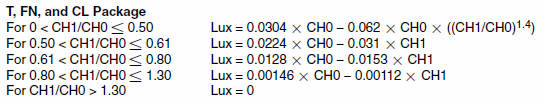
\includegraphics{0_Filer/Figuer/5_HW_Design/Kombinerings_formler.png}
    \caption{Kombinerings formler}
    \label{fig:HWD_Lumen_formler}
\end{figure}

\subsubsection{Afstandssensor}

Den valgte afstandssensor til projektet er af typen HC-SR04. Sensoren er en ultralyds sensor, som bruger sonar til kontaktfri afstandsmåling. Sensorens arbejdsfrekvens ligger på 40 kHz og output er et TTL signal.

Sensoren har 4 ben, VCC, GND, Trig og Echo som vist på billedet.

\begin{figure}[H] \centering
    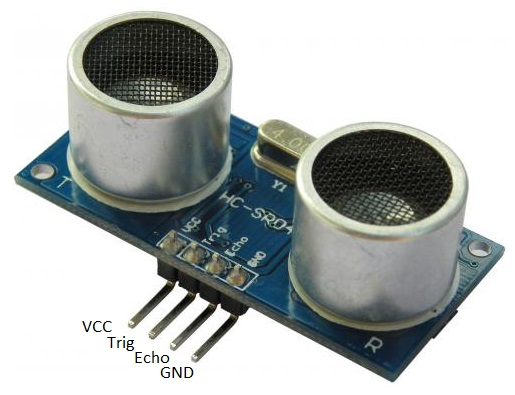
\includegraphics{0_Filer/Figuer/5_HW_Design/HC-SR04.jpg}
    \caption{HC-SR04 afstandssensor}
    \label{fig:HWD_SR04}
\end{figure}

Sensoren har en opløsning på 0,3 cm og er stabil og præcis i intervallet 2 cm til 400 cm, og måler i en vinkel på 15$^{\circ}$. Sensoren skal aktiveres med en TTL puls på mindst 10 mikrosekunder ind på Trig benet. Output fra sensoren kommer som et TTL signal på Echo benet, der har samme længde som tiden fra udsendt sonar burst til ekkosignal modtages af sensoren.

HC-SR04 skal forsynes med 5 VDC, har en idle current på under 2 mA og en working current på 15 mA.

Omregning af output fra sensoren til afstand i cm gøres på følgende måde:

$$Dist(cm) = (\frac{HighLevelTime(s)*340(\frac{m}{s})}{2})*100$$

Forhold mellem trigger TTL puls, sonar burst og TTL ekko kan ses på Timing diagrammet herunder.

\begin{figure}[H] \centering
    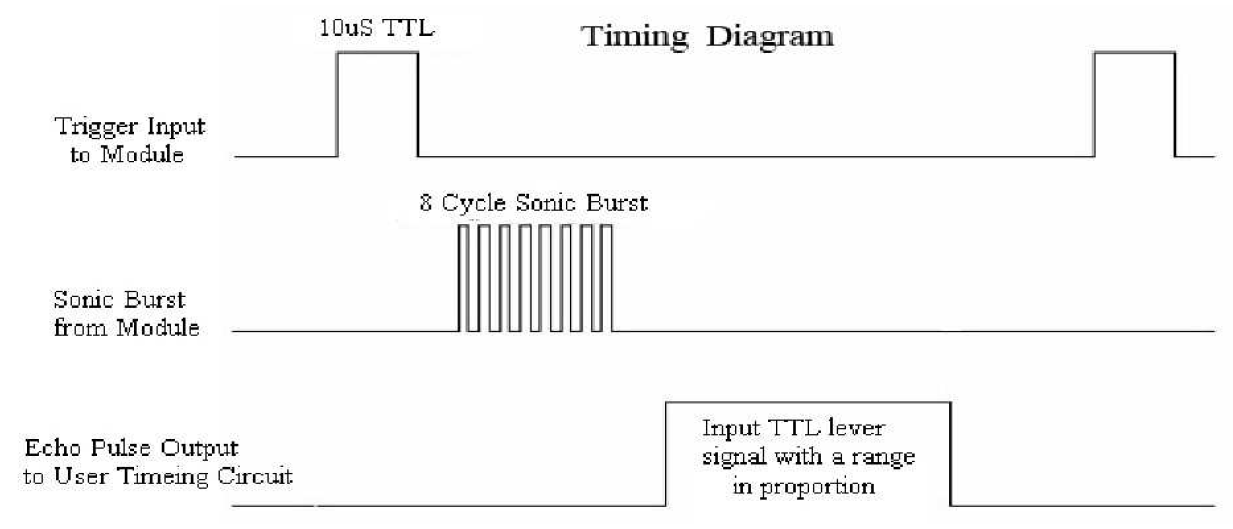
\includegraphics[width=\linewidth]{0_Filer/Figuer/5_HW_Design/HC-SR04_Ultra_Sonic_Timing_Diagram.PNG}
    \caption{HC-SR04 timing diagram}
    \label{fig:HWD_SR04_timing}
\end{figure}

\subsubsection{Bevægelses sensor (PIR)}

Den valgte PIR sensor til projektet er af typen HC-SR501. Sensoren har 3 ben -  VCC, GND og et digitalt output ben. HC-SR501 skal have en forsyningsspænding på mellem 5 og 20 VDC og bruger 65mA. Det digitale output er med TTL standard, hvor High = 3,3V og Low = 0V. HC-SR501 har en justerbar forsinkelse på mellem 0,3 og 5 min. Samt mulighed for at justere max-sensor range fra 3 til 7 m. Både delay og range stilles ved hjælp af hver deres potentiometer.

Ved opstart af modulet vil modulet udsende TTL high 0-3 gange i løbet af det første minut, og derefter gå i standby. Herefter er modulet klar.

Der er mulighed for at sætte sensoren op i to modes ved hjælp af en jumper. Non-repeatable trigger og Repeatable trigger.

Non-repeatable trigger: Når sensoren aktiveres går output benet høj i det interval, der er indstillet med delayet, derefter går benet lavt igen. Benet bliver ikke holdt højt ved gentagen bevægelse, men kan først trigges igen, når det er gået lavt.

Repeatable trigger: Når sensoren aktiveres går output benet højt, og så længe der fortsat er bevægelse vil benet forblive højt. Når bevægelse ophører, vil benet forblive højt til delayet er slut og derefter gå lavt.

\begin{figure}[H]
\centering
\begin{minipage}{.6\textwidth}
  \centering
    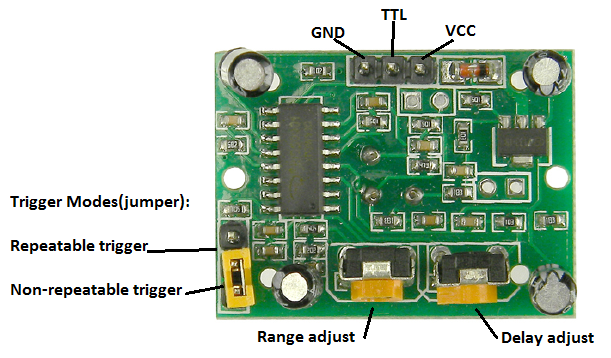
\includegraphics[width=\linewidth]{0_Filer/Figuer/5_HW_Design/HC-SR501_PIR_Motion_Detector_image.png}
    \caption{HC-SR501 PIR sensor}
    \label{fig:HWD_SR501}
\end{minipage}%
\begin{minipage}{.4\textwidth}
  \centering
    \begin{tabular}{ | l | l | }
        \hline
        \textbf{PSoC} & \textbf{HC-SR501} \\ \hline
        GND & GND \\ \hline
        5 V & Vcc \\ \hline
        P2\textunderscore{}0 & TTL \\
        \hline
    \end{tabular}
    \caption{Portforbindelser}
    \label{fig:HWD_PIR_ports}
\end{minipage}
\end{figure}

\subsubsection{5V Stepper motor}

\begin{figure}[H]
\centering
\begin{minipage}{.5\textwidth}
  \centering
  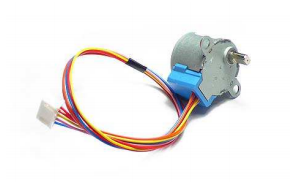
\includegraphics[width=\linewidth]{0_Filer/Figuer/5_HW_Design/Stepper_motor.png}
  \caption{5V stepper motor}
  \label{fig:HWD_Stepper_Motor}
\end{minipage}%
\begin{minipage}{.5\textwidth}
  \centering
  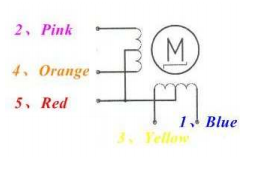
\includegraphics[width=\linewidth]{0_Filer/Figuer/5_HW_Design/Motor_diagram.png}
  \caption{Intern forbindelse i motoren}
  \label{fig:HWD_Stepper_Diagram}
\end{minipage}
\end{figure}

Til styring af X,Y og Z retning benyttes en 5V stepper motor af typen 28BYJ-48 \footcite{28BYJ-48-5V}. Motoren er et oplagt valg, siden den er let tilgængelig på embedded stock, og da den lever op til de krav, som er til systemet. Yderligere er 28BYJ-48-motoren mere kompatibel med det størrelsesforhold prototypen bygges i. Der udover er motorens præcision fordelagtig for projektet, da den har en gearing på 64x48. Dvs. at der er 3072 steps pr. omgang, som gør at lampen kan positioneres meget præcist.

\begin{figure}[H] \centering
    \fbox{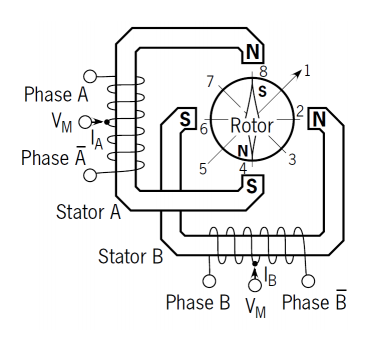
\includegraphics[width=.6\textwidth]{0_Filer/Figuer/5_HW_Design/Bipolar_motor_diagram.png}}
    \caption{Stepper motor}
    \label{fig:HWD_Bipolar_Stepper_Motor}
\end{figure}

Forklaringen herunder tager udgangspunkt i Stator A.
\newline Motoren består af 2 statorer med en nord- og en sydpol. Hver stator har viklinger med to ende tilslutninger, phase A og phase A’, mellem de to ende tilslutninger tilsluttes en 5VDC spænding(Vm). Se figur \ref{fig:HWD_Bipolar_Stepper_Motor}.
Ved at tilslutte phase A til stel, vil strømmen bevæge sig fra Vm til phase A gennem viklingerne, denne bevægelse vil danne et magnetfelt, hvor nord og sydpolen er som på figur \ref{fig:HWD_Bipolar_Stepper_Motor}. Ved tilslutning af phase A’ vil strømmen bevæge sig i modsat retning og de to poler vil bytte plads. Dette gælder også for stator B. Når polerne skifter vil rotorens poler i motoren blive henholdsvis tiltrukket og afvist af statorens poler. \footcite{gfv}

\subsubsection{Micro switch}

\begin{figure}[H]
\centering
\begin{minipage}{.5\textwidth}
  \centering
  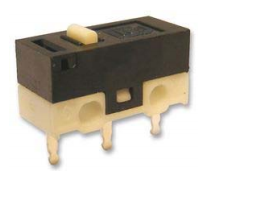
\includegraphics[width=\linewidth]{0_Filer/Figuer/5_HW_Design/Micro_switch.png}
  \caption{Micro Switch (DM1-01P-30-3) \footcite{DM1-01P-30-3}}
  \label{fig:HWD_Micro_switch}
\end{minipage}%
\begin{minipage}{.5\textwidth}
  \centering
  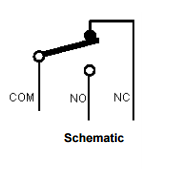
\includegraphics[width=\linewidth]{0_Filer/Figuer/5_HW_Design/Micro_switch_diagram.png}
  \caption{Forbindelses diagram af micro switch \footcite{DM1-01P-30-3}}
  \label{fig:HWD_Micro_Diagram}
\end{minipage}
\end{figure}

Til håndtering af ende stop og kalibrering af X-,Y- og Z-retninger, installeres 5 micro switches(DM1-01P-30-3) \footcite{DM1-01P-30-3}. To switches placeres i enderne på X-skinnen, to på Y-skinnens ender og en ved lampens top-position. Ved aktivering af en af micro switches sættes en port høj på den tilhørende PSoC4, som vil stoppe den bevægelse der nu er nået enden.
Micro switchen forbindes som en NO(normaly open) switch med 5V på COM benet og NO benet forbundet til PSoC4. Se \ref{fig:HWD_Micro_Diagram}.
Iflg. Databladet er micro switchen rated 5V DC og 30mA.

\subsubsection{Strømforbrug}

En enkelt motor bruger 150 mA, når den ikke drejer. Strømforbruget falder når motoren kører. PSoC-XY kommer derfor til at levere mest strøm, da den forsyner 4 motorer, altså 4x 150 mA, og dermed 600 mA hvilket ikke er noget problem for en PSoC. PSoC-Sensor vil levere næstmest strøm i størrelsesordenen 260 mA, beregnet samlet ud fra de forskellige sensorer og LED’er som skal drives af PSoC’en. PSoC-Z levere kun strøm til én motor, hvilket bliver 150 mA.

\subsubsection{Motorstyring}

Et styringsprint er lavet til positionering af vores stepper-motorer. Dette er valgt for at lave en samlet printboks bestående af prints og PSoC’s i vores system. På denne måde kan diverse ledninger, der ellers ville ligge rodet oven i hinanden, blive pakket kompakt i en mere æstetisk behagelig kasse.

\begin{figure}[H] \centering
    \fbox{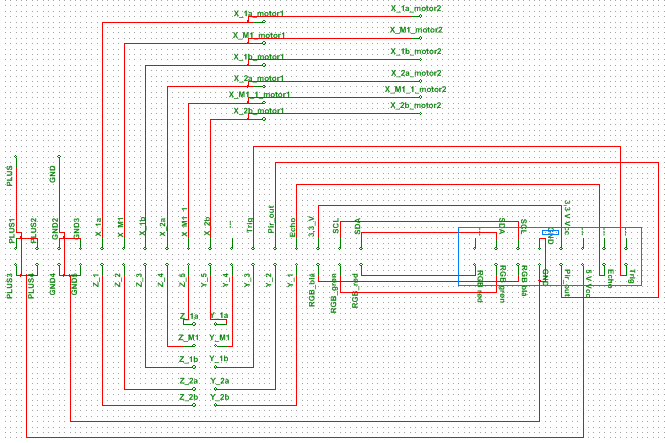
\includegraphics[width=\textwidth]{0_Filer/Figuer/5_HW_Design/XVogn.PNG}}
    \caption{X-Motor Monteringsboard}
    \label{fig:XVogn}
\end{figure}

Kommunikationen går fra de styrende prints gennem et 34-lederkabel og ud til aktuatorerne. På Figur \ref{fig:XVogn} ses et diagram for udlægget af 34-lederkablet. I forsyningskredsløbet sendes der et input ind fra den styrende PSoC, som da bliver forstærket igennem en MosFet. Herefter bliver det sendt ud på 34-lederkablet og går op i et splitterprint i vognene på X- og Y-aksen. Fra disse splitterprints, går signalet direkte ud til steppermotorerne. 


\subsubsection{Print layout}

Systemet består af tre vero printboards et Unified Board(Figur \ref{fig:UniBoard}), et X-Motor Monteringsboard(Figur \ref{fig:XVogn1}) og et YZ-Motor Monteringboard(Figur \ref{fig:YZVogn}).

% Unified Board
\begin{figure}[H] \centering
    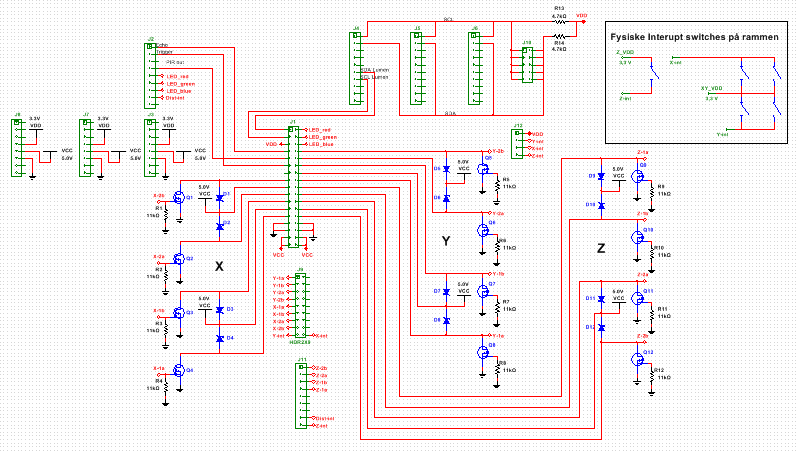
\includegraphics[width=\linewidth]{0_Filer/Figuer/5_HW_Design/UnifiedBoard.PNG}
    \caption{Unified Board}
    \label{fig:UniBoard}
\end{figure}
Dette printboard indeholder de tre motorstyringer til X, Y og Z, hardwaren til I2C kommunikationen og forbinder systemet med PSoC-Master, -XY, -Z og -Sensor.

% X Vogn
\begin{figure}[H] \centering
    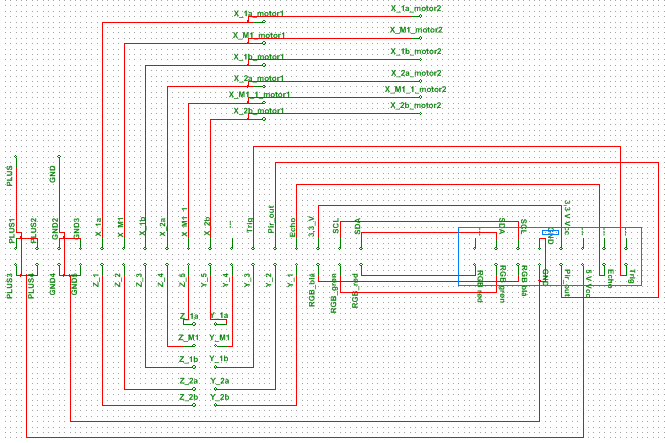
\includegraphics[width=\linewidth]{0_Filer/Figuer/5_HW_Design/XVogn.PNG}
    \caption{X-Motor Monteringsboard}
    \label{fig:XVogn1}
\end{figure}
Dette printboard indeholder X-motor monteringen samt forbindelserne videre ud i systemet.

% YZ Vogn
\begin{figure}[H] \centering
    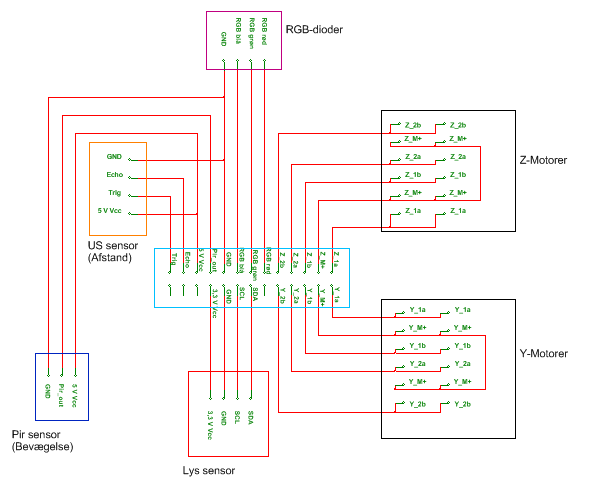
\includegraphics[width=\linewidth]{0_Filer/Figuer/5_HW_Design/YZVogn.PNG}
    \caption{YZ-Motor Monteringsboard}
    \label{fig:YZVogn}
\end{figure}
Dette printboard indeholder YZ-motor monteringerne, forbindelser til PIR-, Lumen- og afstands- sensorerne og RGB dioderne.